% ---------- SECTION IV - FIDO2 & WebAuthn ----------

\section{Results}
\label{sec:results}

To answer the research question, the literature is analyzed for two main topics: usability and security.\\
While there is some amount of research regarding the usability of \ac{fido2}, literature regarding the preceding protocols \ac{u2f} and \ac{uaf} is also taken into account due to the similarity of the involved hardware and authentication flows.\\
The security part of this chapter is mainly based on evaluations of the proposed concepts and mechanisms, as there is not yet any research regarding the security of actual implementations of either hardware or protocols.

% ---- Subsection Usability ----
\subsection{Usability}
\label{subsec:usability}

To determine whether a new authentication concept is accepted by users, and could therefore replace passwords, the usability plays a significant role. Regular passwords have been the prevalent authentication mechanism since the 1960's \cite{mcmillan2012}, so users are very familiar with their usage. The concept of sending credentials, checking them, and granting access to the protected ressource is also very intuitive. Using a hardware token, or in case of internal authenticators only a system dialogue, is a radically different approach.\\
A good starting point to evaluate whether this hardware-dependent approach is suitable is the study conducted by Lang et al \cite{lang2017}. The authors analyzed the roll-out of hardware tokens for 50,000 employees of Google as a second factor.

\textbf{Negative:}
\begin{description}
    \item[Setup complex] 
    \item[Requires hardware] 
    \item[Support of other devices] 
\end{description}

\textbf{Positive:}
\begin{description}
    \item[No memory effort] 
    \item[No phisical effort] 
    \item[Easy key revocation] 
\end{description}

% - Users accept 1FA security tokens
% - Hard/Impossible to use with public computers (no way to insert authenticator)
% - Impossible to delegate access to trusted persons
% - Loosing/Destroying Key -> no access, complicated recovery
%  - Register 2 keys (see: Google Advanced Protection\footnote{https://landing.google.com/advancedprotection/})\cite{gomi2019} or re-run identity checks
% - Many studies for U2F: 25, 26, 39, 40, 41
%  - J. Lang, A. Czeskis, D. Balfanz, M. Schilder, and S. Srinivas, “Security keys: Practical cryptographic second factors for the modern web”
%  - S. Das, G. Russo, A. C. Dingman, J. Dev, O. Kenny, and L. J. Camp,“A qualitative study on usability and acceptability of yubico security key”
%  - S. Das, A. Dingman, and L. J. Camp, “Why johnny doesn’t use two factor: A two-phase usability study of the fido u2f security key”
%  - J. Reynolds, T. Smith, K. Reese, L. Dickinson, S. Ruoti, and K. Seamons, “A tale of two studies: The best and worst of yubikey usability”
% - Rollo-Out in professional environment (Google, 50,000 users) as 2F very successful \cite{lang2017}
% - Response to Key very different across demographics \cite{das2018}, confusing concept, esp. unclear instructions
% - Clear setup instructions needed
% - Form factor especially relevant for older generation

% - Users want to revoke keys -> loss of key associated with loss of account
% - Completely different approach, breaking changes -> Users cannot evaluate the security of this concepts


% ---- Subsection Security ----
\subsection{Security}
\label{subsec:security}

From a security point of view we can mainly analyze the concepts behind the protocols in the \ac{fido2} framework, as there is not yet any research regarding actual protocol implementations or hardware. Therefore, this section is mainly based on the official documentation and first evaluations of security researches. Additionally, we will look mostly at using \ac{fido2} in the passwordless, single factor mode.\\
The main difference to standard passwords is the use of public-key-cryptography instead of storing a shared secret. For every new application the authenticator generates a separate key pair, of which only the public key is stored within the \acp{rp} servers. This has two implications: First, different credentials are used for every service, which means accounts cannot be linked across services based on the key, and as the user has no influence on the key generation, there is no way to derive user information from the public key. Second, as no secret is stored on the RPs side, a credential leak has no effect - knowing the public key is of no use for taking over an account. In addition to that resilience against credential leaks, the public-key infrastructure also prevents against phishing. Even if, for example, a malicious website could forge a \ac{fido2} authentication challenge using stolen public keys, the challenge response can not be used to login to the real account.
% - Public-Key-Cryptography
% - No Phishing, Replay or data breaches possible
% - Keys are Read-Only
% - Require physical presence or even PIN/Biometrics
% - NO resilience to theft
% -> Hardware key can be secured using PIN/Fingerprint, adding knowledge/inheritance factor


% ---- Subsection Other ----
\subsection{Comparison}
\label{subsec:comparison}

The below comparison of passwords, FIDO2 passwordless login and FIDO U2F is based on the authentication method evaluation framework developed by Bonneau et al \cite{bonneau2012}. The evaluation of simple passwords, also proposed by the former authors and supported by others \cite{lyastani2020} is not changed.

\begin{figure*}[ht]
    \centering
    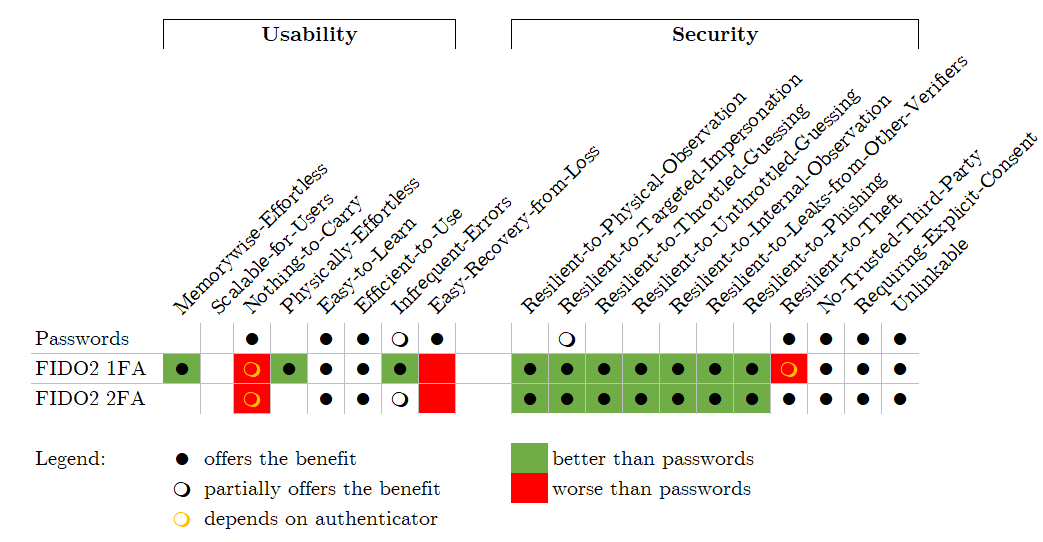
\includegraphics[width=1.8\columnwidth]{Figures/bonneau_matrix.png}
    \caption[Comparison of Authentication Methods]{Comparison of standard passwords with FIDO 1FA/2FA using a modified version of the framework proposed by Bonneau et al (2012)}
    \label{fig:bonneau_matrix}
\end{figure*}

\noindent As figure \ref{fig:bonneau_matrix} shows, both \ac{fido2} modes score exceptionally well. In fact, as is also mentioned in \cite{lyastani2020}, no other authentication method offers as many benefits as the former.